% \chapter{Supplementary Material on Extragalactic Cluster Searches}

\chapter{$J$- and $D$-factors for Extragalactic Sources}
\label{app:JDrelations}

\lettrine[lines=3]{I}{n} this Appendix, we derive the $J$-factor relations used in the main text. We also derive the corresponding $D$-factor relations, which apply to the case of decaying DM.  Although we do not make use of the decay results in the main text, we include these results for completeness because much of our main analysis can be extended to the decaying case.
This Appendix is broken into three subsections. In the first of these, we detail the units and conventions used in our definition of the $J$- and $D$-factors.  After this, we derive an approximate form of the astrophysics factors for different DM density profiles and discuss the accuracy of the approximations made.  We conclude with a discussion of error propagation in the $J$-factors.  Note that several of the details presented in these appendices have been discussed elsewhere, see \emph{e.g.}, Ref.~\cite{Abdo:2010ex,Charbonnier:2011ft,Charbonnier:2012gf,Evans:2016xwx}. 

\section{Units and Conventions}

\subsection{Dark Matter Flux}

We begin by carefully outlining the units associated with the $J$- and $D$-factors. 
The flux, $\Phi$, associated with either DM annihilation or decay factorizes into two parts:
\begin{equation}\begin{aligned}
\frac{d\Phi^{\rm ann.}}{dE_{\gamma}} &= \frac{d\Phi_\text{pp}^{\rm ann.}}{dE_{\gamma}}\times J \, , \\
\frac{d\Phi^{\rm dec.}}{dE_{\gamma}} &= \frac{d\Phi_\text{pp}^{\rm dec.}}{dE_{\gamma}}\times D \, ,
\end{aligned}\end{equation}
where $E_\gamma$ is the photon energy and the `ann.'~(`dec.') superscripts denote annihilation~(decay).  
The particle physics factors are given by:
\begin{equation}\begin{aligned}
\frac{d\Phi_\text{pp}^{\rm ann.}}{dE_{\gamma}} &=\frac{\langle\sigma v\rangle}{8\pi m_{\chi}^{2}}\sum_i \text{Br}_{i}\, \frac{dN_{i}}{dE_{\gamma}}\,, \\
\frac{d\Phi_\text{pp}^{\rm dec.}}{dE_{\gamma}} &=\frac{1}{4\pi m_{\chi} \tau}\sum_i \text{Br}_{i}\, \frac{dN_{i}}{dE_{\gamma}}\,,
\end{aligned}\end{equation}
where $\langle \sigma v \rangle$ is the velocity-averaged annihilation cross section, $m_\chi$ is the DM mass, Br$_i$ is the branching fraction into the $i^\text{th}$ channel, $dN_i/dE_\gamma$ is the photon energy distribution associated with this channel, and $\tau$ is the DM lifetime.  The annihilation factor assumes that the DM is its own antiparticle; if this were not the case, and assuming no asymmetry in the dark sector, then the factor would be half as large.  The particle physics factors carry the following dimensions:
\begin{equation}\begin{aligned}
\left[ \frac{d\Phi_\text{pp}^{\rm ann.}}{dE_{\gamma}} \right] &= {\rm counts} \cdot {\rm cm}^3 \cdot {\rm s}^{-1} \cdot {\rm GeV}^{-3} \cdot {\rm sr}^{-1} \,, \\
\left[ \frac{d\Phi_\text{pp}^{\rm dec.}}{dE_{\gamma}} \right] &= {\rm counts} \cdot {\rm s}^{-1} \cdot {\rm GeV}^{-2} \cdot {\rm sr}^{-1}\,,
\label{eq:ppunits}
\end{aligned}\end{equation}
where `counts' refers to the number of gamma-rays produced in the interaction and the ${\rm sr}^{-1}$ is associated with the $1/4\pi$ in the particle physics factors.  Note that some references include this $4\pi$ in the definition of the $J$- or $D$-factors, but this is not the convention that we follow here.

The $J$- and $D$-factors are defined as follows:
\begin{equation}\begin{aligned}
J &= \left(1+b_\text{sh}[M_\text{vir}]\right)\,\int ds \, d\Omega \,\rho_{\rm DM}^2(s,\Omega) \,, \\
D &= \int ds\, d\Omega\, \rho_{\rm DM}(s,\Omega)\,,
\label{eq:JDdef}
\end{aligned}\end{equation}
where $b_\text{sh}[M_\text{vir}]$ is the subhalo boost factor.  The $J$- and $D$-factors carry the following units:
\begin{equation}\begin{aligned}
\left[ J \right] &= {\rm GeV}^2 \cdot {\rm cm}^{-5} \cdot {\rm sr}\,, \\
\left[ D \right] &= {\rm GeV} \cdot {\rm cm}^{-2} \cdot {\rm sr}\,.
\end{aligned}\end{equation}
Combining these with Eq.~\ref{eq:ppunits}, we find that 
\begin{equation}
\left[ \frac{d\Phi}{dE_{\gamma}} \right] = {\rm counts} \cdot {\rm cm}^{-2} \cdot {\rm s}^{-1} \cdot {\rm GeV}^{-1}\,
\end{equation}
for both the annihilation and decay case.  This means that $\Phi$ is given in units of counts per experimental effective area [${\rm cm}^2$] per experimental run time [${\rm s}$].  
In this work, we study extragalactic objects with small angular extent.  So long as each object is centered on the region-of-interest (ROI), we expect that all of its flux will be contained within the ROI as well.  This means that the photon counts obtained by integrating Eq.~\ref{eq:JDdef} over the entire sky corresponds to the total counts expected from that object in the ROI.  The situation is different when treating objects with a large angular extent that exceeds the size of the ROI---\emph{e.g.}, when looking for emission from the halo of the Milky Way.  In such cases, it is more common to divide the $J$- and $D$-factors by the solid angle of the ROI ($\Delta \Omega$) such that both they, and consequently $\Phi$, are averages rather than totals.  

\subsection{Halo Mass and Concentration}

We briefly comment here on different mass and concentration definitions (virial and 200) as relevant to our analysis.   Boost-factor models, concentration-mass relations, and masses are often specified in terms of 200 quantities, which must be converted to virial ones. In order to do this, we use the fact that
\begin{equation}\begin{aligned}
\frac{\rho_\text{s}}{\rho_c} \equiv \delta_\mathrm{c} = \frac{\Delta_\text{c}}{3}\frac{c^3}{\log{(1+c)}-c/(1+c)}
\label{eq:CritOverdens}
\end{aligned}\end{equation}
for the NFW profile~\cite{Navarro:1995iw}, where $\rho_s$ is the normalization of the density profile, $\rho_c$ is the critical density, $c$ is the concentration parameter, and $\delta_\mathrm{c}$ is the critical overdensity.  For virial quantities, $\Delta_c(z) = 18\pi^2 +82x-39x^2$ with $x = \Omega_{m}(1+z)^3/[\Omega_{m}(1+z)^3 + \Omega_{\Lambda}]-1$ in accordance with Ref.~\cite{Bryan:1997dn}, while for 200 quantities, $\Delta_c = 200$.  Therefore, Eq.~\ref{eq:CritOverdens} can be equated between the 200 and virial quantities and solved numerically to convert between definitions of the concentration.

For different mass definitions, we have 
\begin{equation}\begin{aligned}
\frac{M_{200}}{M_\text{vir}} = \left(\frac{c_{200}[M_{200}]}{c_\text{vir}[M_\text{vir}]}\right)^3\frac{200}{\Delta_\text{c}} \, ,
\label{eq:MassConvert}
\end{aligned}\end{equation}
where the concentration definitions on the right-hand side depend on $M_{200}$ and $M_\text{vir}$ and may have to be converted between each other and we have suppressed the redshift dependence for clarity.  Solving this numerically, we can convert between the two mass definitions.

\section{Approximate $J$- and $D$-factors}

For an extragalactic DM halo, the astrophysical factors in Eq.~\ref{eq:JDdef} can be approximated as:
\begin{equation}\begin{aligned}
J &\approx \left(1+b_\text{sh}[M_\text{vir}]\right)\, \frac{1}{d_c^2[z]} \int_V dV' \rho_{\rm DM}^2(r') \,, \\
D &\approx \frac{1}{d_c^2[z]} \int_V dV' \rho_{\rm DM}(r')\,,
\vspace{0.5in}
\label{eq:JDdapprox}
\end{aligned}\end{equation}
where the integrals are performed in a coordinate system centered on the halo, and $d_c[z]$ is the comoving distance, which is a function of redshift for a given cosmology.  The aim of this subsection is to derive Eq.~\ref{eq:JDdapprox} from Eq.~\ref{eq:JDdef} and to quantify the error associated with this approximation. 

To handle the $J$- and $D$-factors simultaneously, we consider the following integral over all space:
\begin{equation}
\int ds \, d\Omega \,\rho_{\rm DM}^n(s,\Omega)\,,
\end{equation}
with $n \geq 1$. Here, $s$ is playing the role of a radius in a spherical coordinate system centered on the Earth.  Therefore, we can rewrite the measure as
\begin{equation}
\int s^2\, ds \, d\Omega \,\, \frac{\rho_{\rm DM}^n(s,\Omega)}{s^2} = \int dV\, \frac{\rho_{\rm DM}^n(s,\Omega)}{s^2}\,.
\end{equation}

Next, we transform to a coordinate system (denoted by primed quantities) that is centered at the origin of the halo described by $\rho_{\rm DM}$.  Because this change of coordinates is only a linear translation, it does not induce a Jacobian and $dV = dV'$.  Assuming that the Earth is located at a position $\mathbf{r}$ from the halo center and the DM interaction occurs at position $\mathbf{r'}$, then $s = | \mathbf{r} - \mathbf{r}'| $ and
\begin{equation}
\int dV\, \frac{\rho_{\rm DM}^n(s,\Omega)}{s^2} = \int dV'\, \frac{\rho_{\rm DM}^n(r',\Omega')}{r^{\prime 2} - 2 d_c r' \cos \theta' + d_c^2}\,,
\label{eq:haloframe}
\end{equation}
where we take $|\mathbf{r}| = d_c$ and $\mathbf{r} \cdot \mathbf{r}' = d_c\, r' \, \cos\theta'$.

Eq.~\ref{eq:haloframe} can be simplified by taking advantage of several properties of the halo density.  First, it is spherically symmetric about the origin of the primed coordinate system.  Second, it only has finite support in $r'$.  In particular, it does not make sense to integrate the object beyond the virial radius, $r_{\rm vir}$. This allows us to rewrite the integral as follows:
\vspace{0.1in}

\begin{eqnarray}
\label{eq:multiline}
\int dV'\, \frac{\rho_{\rm DM}^n(r',\Omega')}{r^{\prime 2} - 2 d_c r' \cos \theta' + d_c^2}
&=& \int_0^{r_{\rm vir}} dr'\, \int d\Omega'\, \frac{\rho_{\rm DM}^n(r')}{r^{\prime 2} - 2 d_c r' \cos \theta' + d_c^2} \\
&=& \frac{2 \pi}{d_c^2} \, \int_0^{r_{\rm vir}} dr'\, \rho_{\rm DM}^n(r')  \int_0^{\pi} d\theta'\, \frac{\sin \theta'}{1 - 2 (r'/d_c) \cos \theta' + (r'/d_c)^2} \notag \\
&=& \frac{2\pi}{d_c^2} \, \int_0^{r_{\rm vir}} dr'\, \frac{ \rho_{\rm DM}^n(r')}{2\,(r'/d_c)} \ln \left[ \frac{((r'/d_c)+1)^2}{((r'/d_c)-1)^2} \right]\,. \notag
\end{eqnarray}

For extragalactic objects, $d_c \gg r_{\rm vir} \geq r'$.  As a result, we can take advantage of the following  expansion:
\begin{equation}
\frac{1}{2x} \ln \left[ \frac{(x+1)^2}{(x-1)^2} \right]  = 2 \left[ 1 + \frac{1}{3} x^2 + \mathcal{O} \left(x^4\right) \right] \, ,
\label{eq:logexpand}
\end{equation}
where $x= r'/d_c$.  It follows that the leading-order approximation to Eq.~\ref{eq:multiline} is \begin{equation}\begin{aligned}
\int ds \, d\Omega \,\rho_{\rm DM}^n(s,\Omega) = \frac{1}{d_c^2} \int dV' \rho_{\rm DM}^n(r') \,,
\end{aligned}\end{equation}
which when inserted into Eq.~\ref{eq:JDdef} gives Eq.~\ref{eq:JDdapprox}, as claimed. 

We can calculate the size of the neglected terms in Eq.~\ref{eq:logexpand} to quantify the accuracy of this approximation.  We take the parameters of the halo with the largest $J$-factor in the catalog to estimate the largest error possible amongst the \texttt{DarkSky} halos.  For this halo, the fractional correction to the $J$-factor of the first neglected term in the expansion is $\mathcal{O}(10^{-5})$ for either an NFW or Burkert profile (described below), whilst for the $D$-factor it is $\mathcal{O}(10^{-4})$. These values are significantly smaller than the other sources of uncertainty present in estimating these quantities and so we conclude that the approximations in Eq.~\ref{eq:JDdapprox} are sufficient for our purposes.



\section{Analytic Relations}

Starting from the approximate forms given in Eq.~\ref{eq:JDdapprox} and specifying a DM density profile $\rho_{\rm DM}$, the $J$- and $D$-factors can often be determined exactly.   We will now demonstrate that the final results only depend on the distance, mass, and concentration of the halo---for a given substructure boost model and cosmology.

As a starting point, consider the NFW profile:
\begin{equation}
\rho_{\rm NFW}(r) = \frac{\rho_s}{r/r_s(1+r/r_s)^2}\,.
\end{equation}
The parameter $r_s$ is the scale radius and dictates how sharply peaked the core of the DM distribution is.
Starting from this distribution, the volume integral in the $J$-factor evaluates to
\begin{equation}\begin{aligned}
\int dV'\, \rho_{\rm NFW}^2(r') &= 4\pi \rho_s^2 r_s^2 \int_0^{r_{\rm vir}} \frac{dr'}{(1+r'/r_s)^4} \\
&= \frac{4\pi}{3} \frac{\rho_s^2 r_{\rm vir}^3}{c_{\rm vir}^3} \left[ 1 - \frac{1}{(1+c_{\rm vir})^3} \right]\,,
\label{eq:NFWVolumeInt}
\end{aligned}\end{equation}
where $c_{\rm vir} = r_{\rm vir}/r_s$ is the virial concentration.  To remove the normalization factor $\rho_s$ from this equation, we can write the virial mass of the halo as
\begin{equation}\begin{aligned}
M_{\rm vir} &\equiv \int dV'\, \rho_{\rm NFW}(r') \\
&= 4\pi \rho_s \frac{r_{\rm vir}^3}{c_{\rm vir}^3} \left[ \ln \left( 1 + c_{\rm vir} \right) - \frac{c_{\rm vir}}{1+c_{\rm vir}} \right]\,,
\end{aligned}\end{equation}
which, when combined with Eq.~\ref{eq:NFWVolumeInt}, gives
\begin{equation}\begin{aligned}
\int dV'\, \rho_{\rm NFW}^2(r)
=\,&\frac{M_{\rm vir}^2 c_{\rm vir}^3}{12\pi r_{\rm vir}^3} \left[ 1 - \frac{1}{(1+c_{\rm vir})^3} \right] \\
\times &\left[ \ln \left( 1 + c_{\rm vir} \right) - \frac{c_{\rm vir}}{1+c_{\rm vir}} \right]^{-2}\,.
\end{aligned}\end{equation}
Stopping here, we would conclude that the $J$-factor scales as $M_{\rm vir}^2$.  However, for a given $M_{\rm vir}$ and cosmology, $r_{\rm vir}$ is not an independent parameter. Using the results of Ref.~\cite{Bryan:1997dn}, we can write:
\begin{equation}
\frac{3M_{\rm vir}}{4\pi r_{\rm vir}^3} = \rho_c \Delta_c[z]\,,
\end{equation}
where $\rho_c$ is the critical density and 
\begin{equation}\begin{aligned}
\Delta_c[z] &\equiv  18\pi^2 + 82\,x[z] - 39\,x[z]^2\,, \\
x[z] &\equiv \frac{\Omega_m \left( 1 + z \right)^3}{\Omega_m \left( 1 + z \right)^3 + \Omega_{\Lambda}} - 1\,.
\end{aligned}\end{equation}
This relation can then be used to remove $M_{\rm vir}/r_{\rm vir}^3$ from the volume integral and we conclude that
\begin{align}
J_{\rm NFW} \approx &\left(1+b_\text{sh}[M_\text{vir}]\right) \frac{M_{\rm vir} c_{\rm vir}^3 \rho_c \Delta_c[z]}{9 d_c^2[z]} \label{eq:JNFWfull} \\
\times &\left[ 1 - \frac{1}{(1+c_{\rm vir})^3} \right] \left[ \ln \left( 1 + c_{\rm vir} \right) - \frac{c_{\rm vir}}{1+c_{\rm vir}} \right]^{-2}\,. \notag
\end{align}
We see the additional mass dimension required from the fact this scales as $M_{\rm vir}$ not $M_{\rm vir}^2$ is carried by $\rho_c$. The $c_{\rm vir}^3$ dependence highlights that the annihilation flux is critically dependent upon how sharply peaked the halo is.   To summarize, Eq.~\ref{eq:JNFWfull} demonstrates that the $J$-factor is fully specified by three halo parameters for a given substructure boost model and cosmology: the redshift $z$, mass $M_{\rm vir}$, and concentration $c_{\rm vir}$.

%\begin{figure*}[t]
%   \centering
%   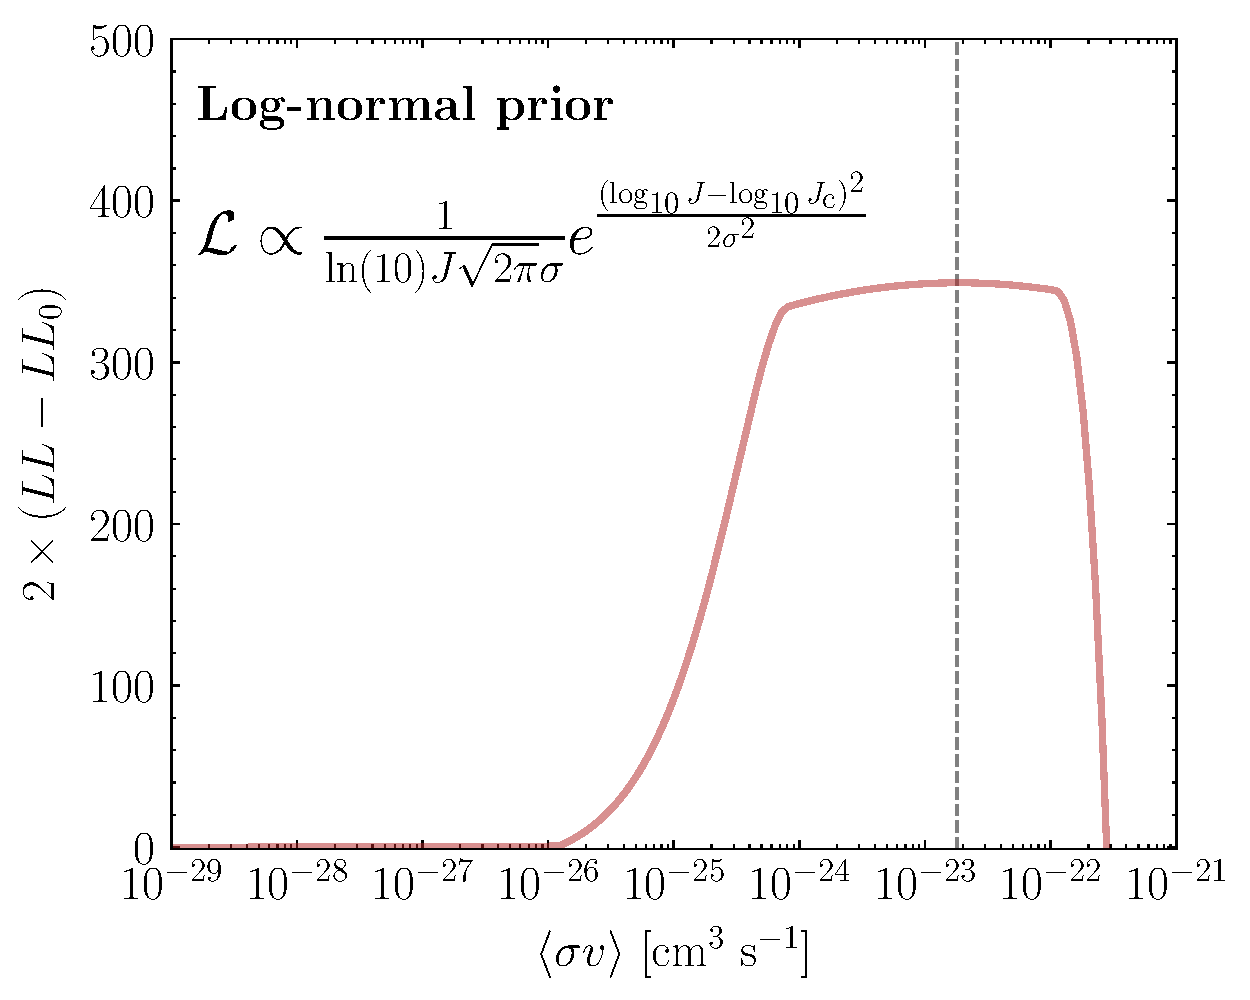
\includegraphics[width=0.45\textwidth]{ch-darksky/plots//jfactor_wrongLL.pdf}  ~\hspace{2mm}
%   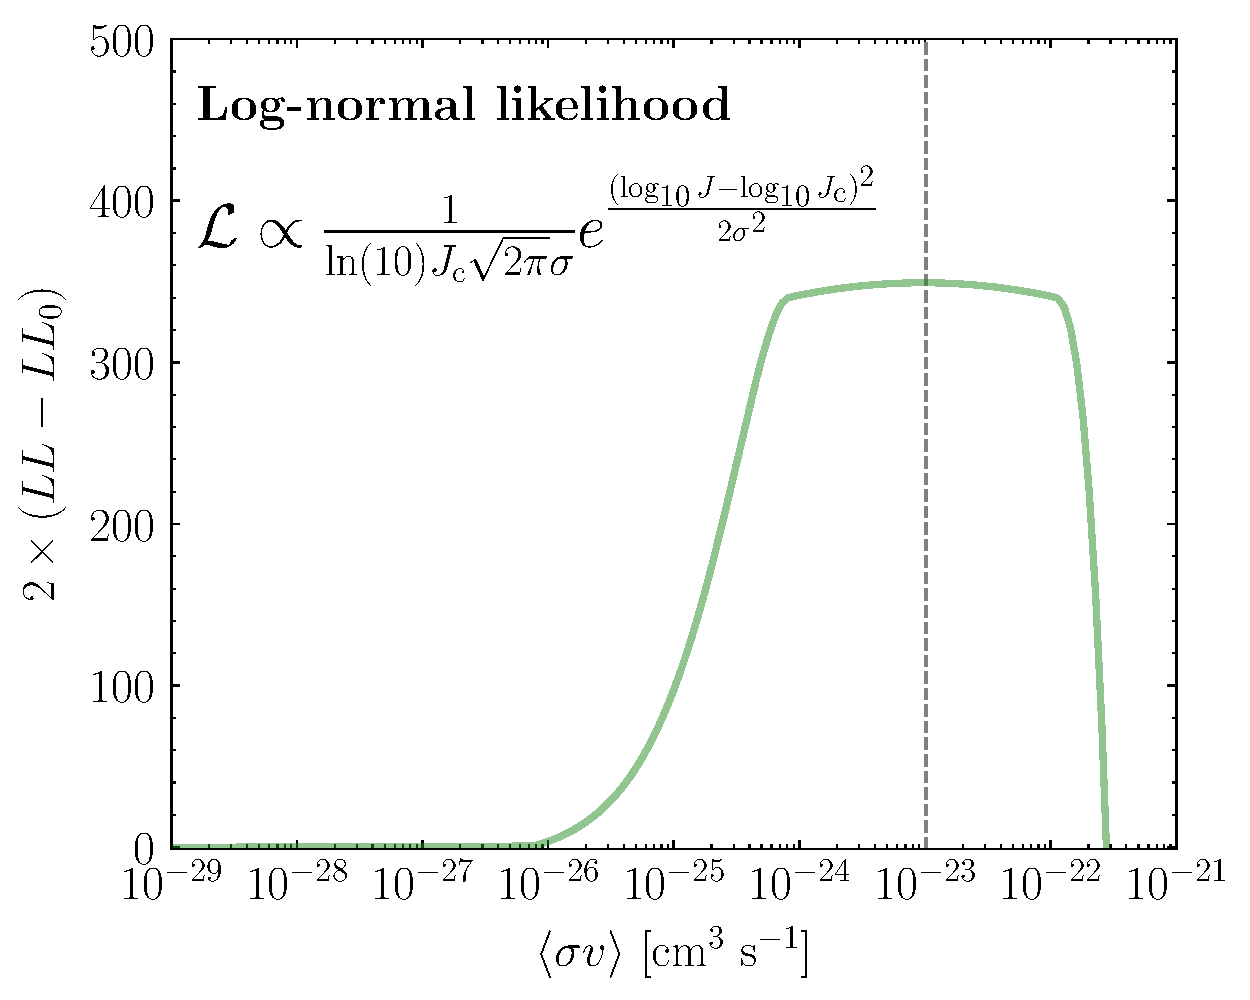
\includegraphics[width=0.45\textwidth]{ch-darksky/plots//jfactor_correctLL.pdf} 
%   \caption{Impact of using the log-normal prior for the $J$-factor \textbf{(Left)} versus using the log-normal likelihood \textbf{(Right)}.  This is illustrated by showing the test statistic as a function of cross section for a single halo after injecting a DM signal of $\langle\sigma v \rangle= 10^{-23}\,{\rm cm}^3\,{\rm s}^{-1}$ at $m_\chi =100$ GeV. The recovered cross section is   associated with the maximum of the test statistic and is indicated by the vertical dashed line. The log-normal likelihood on the right correctly recovers the injected signal, while the log-normal prior on the left inevitably leads to an offset with respect to the underlying signal strength. Note that true, rather than inferred, $J$-factors are used in this case for illustration.}
%   \label{fig:LLJfacForms}
%\end{figure*}

The basic scalings and dependence shown above are not peculiar to the NFW profile, but are in fact more generic. To demonstrate this, we can repeat the above exercise for the cored Burkert profile~\cite{Burkert:1995yz}:
\begin{equation}
\rho_{\rm Burkert}(r) = \frac{\rho_B}{(1+r/r_B)(1+(r/r_B)^2)}\,,
\end{equation}
which is manifestly non-singular as $r \to 0$ unlike the NFW profile.  Here, $\rho_B$ and $r_B$ are the Burkert analogues of $\rho_s$ and $r_s$ in the NFW case, but they are not exactly the same.  Indeed, following \emph{e.g.}, Ref.~\cite{Bartels:2015uba}, by calculating physically measurable properties of halos such as the radius of maximum rotational velocity for both the NFW and Burkert cases and setting them equal, we find
\begin{equation}
r_B \simeq 0.7 r_s\,.
\end{equation}
We will replace $r_B$ with a concentration parameter $c_B = r_{\rm vir}/r_B$.  Following the same steps as for the NFW profile, we arrive at:
\begin{align}
J_{\rm Burkert} \approx &\left(1+b_\text{sh}[M_\text{vir}]\right) \frac{4M_{\rm vir} c_B^3 \rho_c \Delta_c[z]}{3 d_c^2[z]} \\
\times &\left[ \frac{c_B(1+c_B+2c_B^2)}{(1+c_B)(1+c_B^2)} - \arctan(c_B) \right] \notag \\
\times &\left[ \ln \left[ (1+c_B)^2 (1+c_B^2) \right] - 2 \arctan(c_B) \right]^{-2}\,, \notag
\end{align}
from which we see that $J \sim (1+b_\text{sh}) M_\text{vir} c_B^3\rho_c/d_c^2[z]$.

For the case of decaying DM, the approximate integral given in Eq.~\ref{eq:JDdapprox} can be evaluated independent of any choice for the halo profile.   Specifically:
\begin{equation}\begin{aligned}
D &\approx \frac{1}{d_c^2[z]} \int_V dV' \rho_{\rm DM}(r) = \frac{M_{\rm vir}}{d_c^2[z]}\,,
\label{eq:Dfactor}
\end{aligned}\end{equation}
where the second equality follows from the fact that the volume integral gives the virial mass exactly.
For DM decays in relatively nearby halos, the emission can be quite extended, as the flux is not as concentrated towards the center of the halo as in the annihilation case.  As such, it is often useful to have a version of the extragalactic $D$-factor where one only integrates out to some angle $\theta$ on the sky from the center of the halo, or equivalently to a distance $R = \theta \cdot d_c(z) < r_{\rm vir}$. In this case:\begin{align}
D &\approx \frac{M_{\rm vir}}{d_c^2(z)} \\
&\times \left[ \ln \left( 1 + \frac{c_{\rm vir} R}{r_{\rm vir}[M_{\rm vir}]} \right) - \frac{c_{\rm vir}}{r_{\rm vir}[M_{\rm vir}]/R + c_{\rm vir}} \right] \notag \\
&\times \left[ \ln (1 + c_{\rm vir}) - \frac{c_{\rm vir}}{1+c_{\rm vir}} \right]^{-1}\,, \notag
\end{align}
for the NFW profile, where we have made explicit the fact that $r_{\rm vir}$ is a function of $M_{\rm vir}$.  When $R=r_{\rm vir}$, this reduces to the simple result in Eq.~\ref{eq:Dfactor}.

% \subsection{Propagating $J$-factor Uncertainties}
% \label{app:Juncertainties}

% We now discuss the propagation of uncertainties from inferred halo parameters into an overall uncertainty on the $J$-factor.  Specifically, we will justify the form of the log-normal distribution for the $J$-factor that was used in Eq.~\ref{eq:Jlognormal} of the main text.  While we focus our attention on the case of the $J$-factor for the NFW profile, the logic carries over straightforwardly to the Burkert profile, or even to the $D$-factor.

% Our starting point is the approximate form of the NFW $J$-factor given in Eq.~\ref{eq:JNFWfull}, which shows that the $J$-factor is determined by the redshift  $z$, mass $M_{\rm vir}$, and concentration $c_{\rm vir}$, for a given substructure boost model and cosmology.  Therefore, the errors on these three parameters need to be propagated to determine the total error on the $J$-factor.  When the redshift $z$ is determined spectroscopically, the uncertainty on $d_c$ is  subdominant to the uncertainties on the $J$-factor that are induced by the mass and concentration. As such, we neglect the uncertainty in the redshift. If one were using photometric redshifts, however, these uncertainties would also need to be accounted for.  Additionally, for nearby halos in particular, the relation between redshift and distance can have further uncertainties, since this relation is affected by local peculiar velocities.  

% From our studies of \texttt{DarkSky}, we see that the $M_{\rm vir}$ and $c_{\rm vir}$ distributions are well-approximated as log-normal. If the $J$-factor simply scaled as the product of several log-normal distributions ($J \sim M_{\rm vir} c_{\rm vir}^3$), then $J$ would also be log-normally distributed.  However, the dependence of the concentration parameter and boost factor on the virial mass mean that $J$ will not be exactly distributed in this way. Nevertheless, by explicitly calculating the full $J[M_{\rm vir}, c_{\rm vir}]$ distribution, we confirm that it is very accurately log-normally distributed. The reason for this is that the mass dependence of the boost factor in the Bartels substructure model~\cite{Bartels:2015uba} is very mild and additionally the $c_{\rm vir}$ dependence is subdominant in dictating the form of $J$, beyond the $c_{\rm vir}^3$ dependence.  Because the log-normal is  considerably simpler than the full distribution, we adopt it for the $J$-factor.

% The form of the likelihood that we use for the $J$-factor in Eq.~\ref{eq:Jlognormal} is the same as that used in Ref.~\cite{Ackermann:2015zua}, but stands in contrast to Ref.~\cite{Ackermann:2011wa,Ackermann:2013yva} with the substitution of the nominal central $J$-factor in the denominator instead of the marginalized value. The interpretation of the $J$-factor as a log-normal likelihood~\cite{Ackermann:2015zua}  rather than a log-normal prior~\cite{Ackermann:2011wa,Ackermann:2013yva} ensures proper normalization for all values of $J$ and, when interpreted as a maximum likelihood estimator for signal recovery, coincides with the true underlying signal strength. This is illustrated in Fig.~\ref{fig:LLJfacForms}, where we show the test statistic as a function of DM cross section obtained for an injected signal of $\langle\sigma v \rangle= 10^{-23}\,{\rm cm}^3\,{\rm s}^{-1}$ at $m_\chi =100$ GeV after $J$-factor marginalization in the two different cases for a single halo. The left panel shows the traditional log-normal prior form of the likelihood.  The maximum of this, indicated by the vertical dotted line, is offset from the true value of the underlying cross section. This discrepancy can be substantially amplified when stacking a large number of objects. Using the log-normal likelihood form (right panel), we see that the maximum test statistic associated with the recovered signal coincides with the injected signal at the true value, $\langle\sigma v \rangle= 10^{-23}\,{\rm cm}^3\,{\rm s}^{-1}$.


% \section{Validity of Likelihood Approximation}
% \label{app:energyrange}

% In this Appendix, we address issues pointed out in the main text where our analysis procedure appears to induce small systematic discrepancies.  First, we discuss the incorporation of the $J$-factor uncertainties, and then we discuss issues related to the profile likelihood procedure itself. 

% \subsection{J-factor Likelihood}

% In Fig.~\ref{fig:DSinjsiglocs} of the main text,  the best-fit cross sections are systematically $\sim1$$\sigma$ higher than their injected values at high $\langle \sigma v \rangle_\text{inj}$ where DM detection is significant.  While this could be consistent with statistical fluctuations in the $J$-factor distributions, it  likely results from the fact that the assumed $J$-factor distributions, and the methods we have for calculating the central values and uncertainties, are not an exact representation of the actual $N$-body data.  To demonstrate this, Fig.~\ref{fig:noJuncertainty} shows the $m_\chi = 10$~TeV injected signal plot for an observer at Location~1, where all $J$-factors are fixed to their true values.  In this case, the best-fit cross section exactly matches the injected cross section at high values of $\langle \sigma v \rangle_\text{inj}$, confirming that it is indeed the assumed $J$-factor distributions that induce the bias seen in Fig.~\ref{fig:DSinjsiglocs}.

% \begin{figure}[t]
%    \centering
%    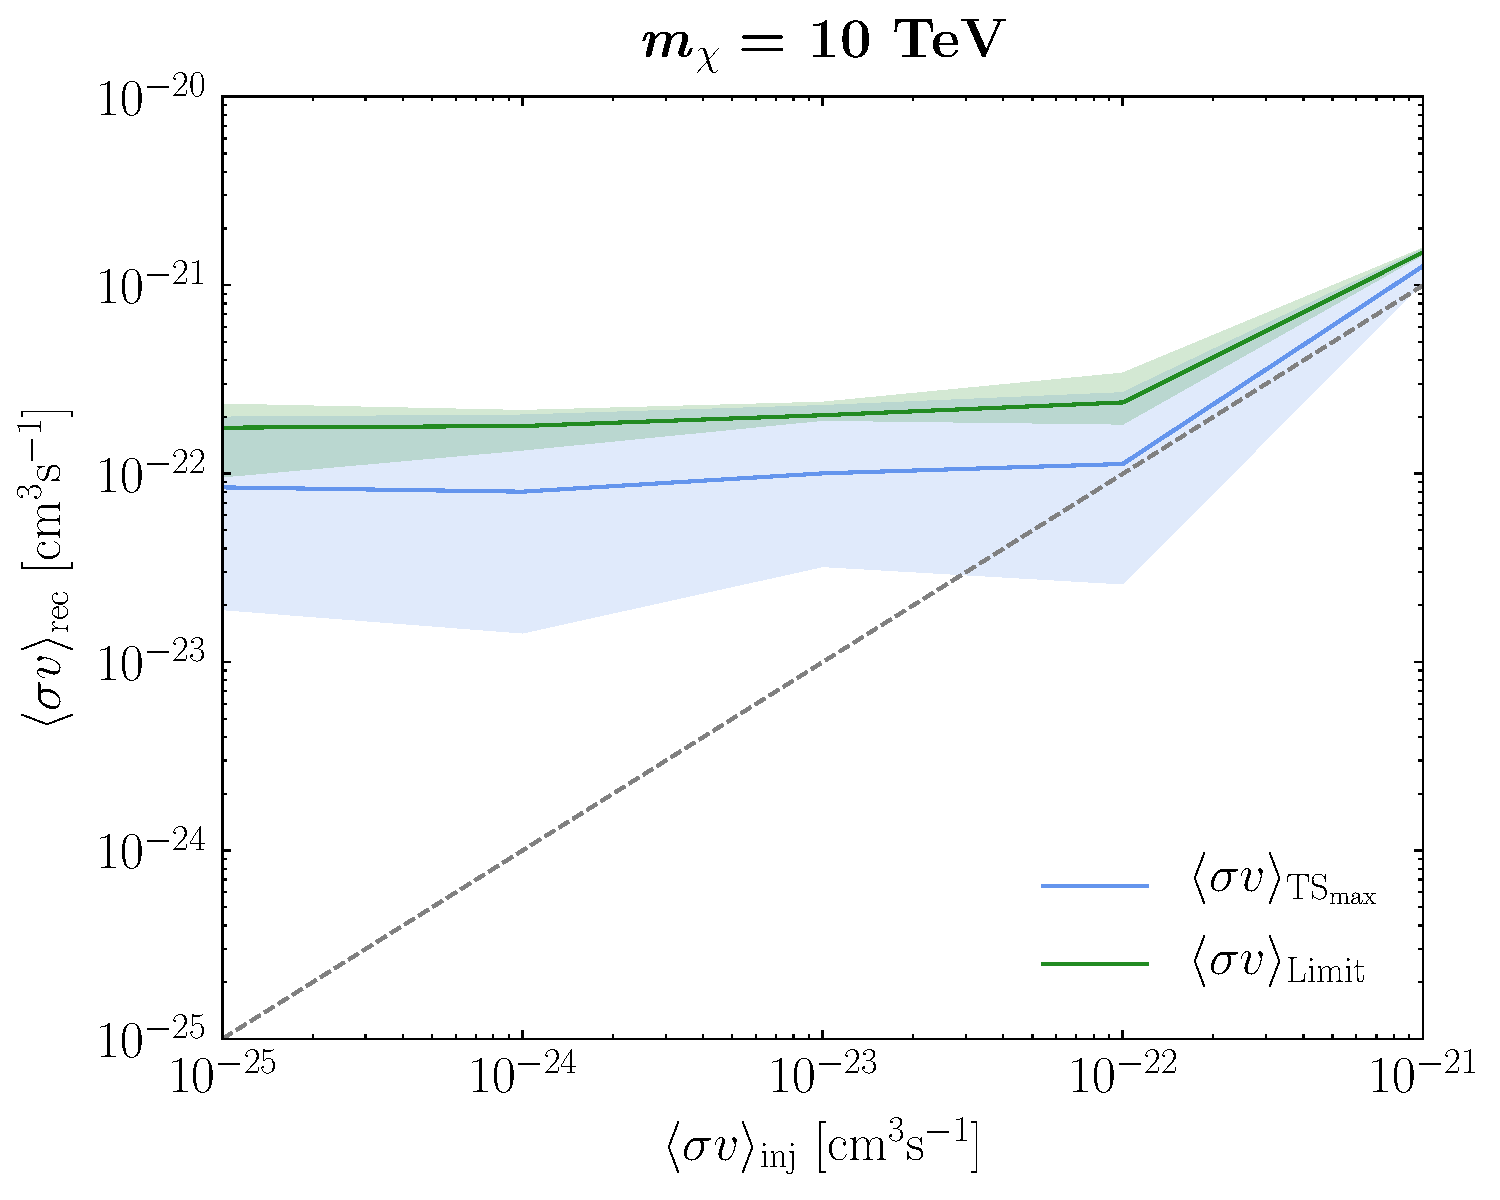
\includegraphics[width=0.48\textwidth]{ch-darksky/plots//signal_recovery_10TeV_noJuncert.pdf} \hspace{0.01cm}
%    \caption{ The same as Fig.~\ref{fig:DSinjsiglocs} for $m_\chi = 10$ TeV and for an observer at Location~1, except that the $J$-factors are fixed to their true values. Contrasting with the analogous plot in Fig.~\ref{fig:DSinjsiglocs}, we see that the $J$-factor uncertainties induce a small bias, at the $1$$\sigma$ level, towards higher recovered cross sections. }
%    \label{fig:noJuncertainty}
% \end{figure}

% \subsection{Profile Likelihood Approximation}
% \begin{figure*}[t]
%    \centering
%    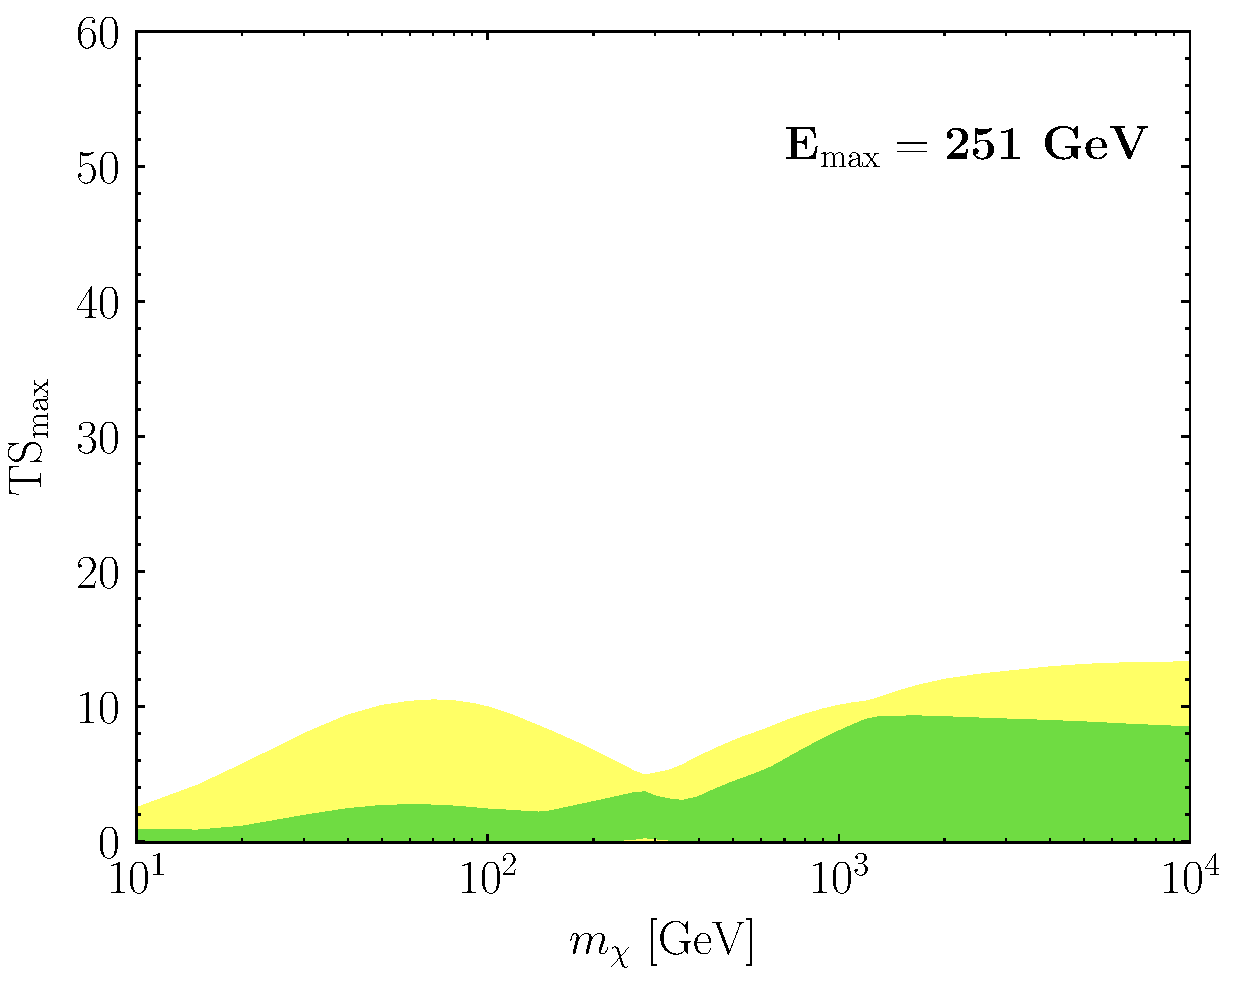
\includegraphics[width=0.45\textwidth]{ch-darksky/plots//global_e251.pdf}
%    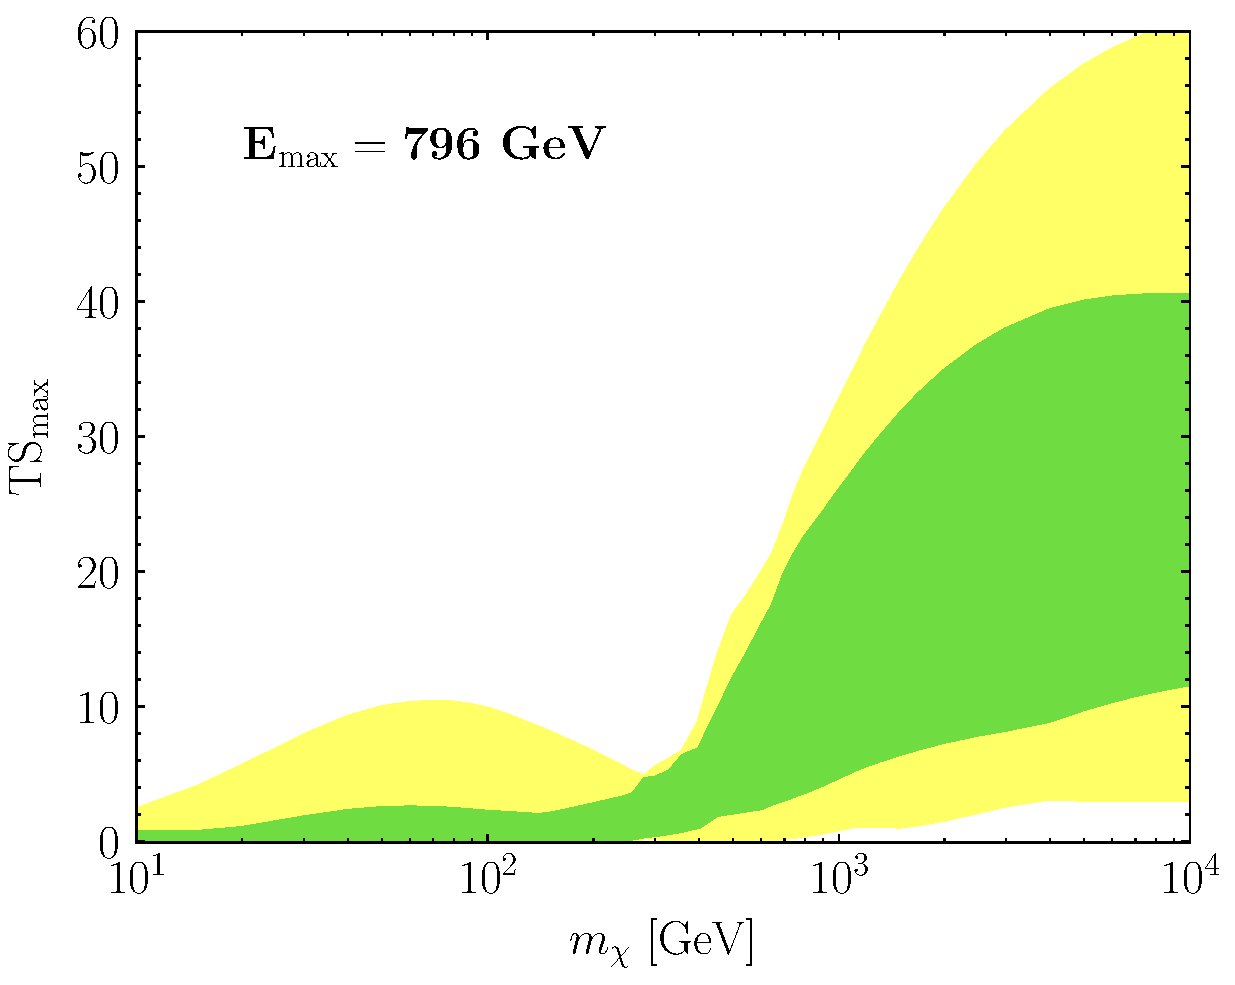
\includegraphics[width=0.45\textwidth]{ch-darksky/plots//global_e796.pdf}   
%    \caption{ Maximum test statistic, TS$_\text{max}$, for the stacked analysis comparing the model with and without DM annihilating to $b \bar b$.  The green~(yellow) bands show the 68\%~(95\%) containment over multiple random sky locations.  The results are shown restricting the analysis to energies below 251 \textbf{(Left)} and 796 \textbf{(Right)}~GeV.  In both cases, the minimum energy is 500 MeV.}
%    \label{fig:LikelihoodApprox}
% \end{figure*}

% As described in Sec.~\ref{sec:stats}, we use an approximation  to the full profile likelihood procedure to make the analysis computationally tractable.  This approximation comes into play when removing the nuisance parameters associated with the astrophysical templates:
% \begin{equation}
% \mathcal{L}_i^r(d_i^r | \psi_i, J^r) = \max_{\{\lambda_i^r\}}\,\mathcal{L}_i^r \left( d_i^r | \boldsymbol{\theta}_i^r, J^r \right)\,,
% \label{eq:firstprofileSM}
% \end{equation}
% following the notation of Sec.~\ref{sec:stats}.  To briefly review, the full implementation of the profile likelihood requires maximizing the $\lambda_i^r$ for all $\psi_i$ and $J^r$.  Instead, we set the $\lambda_i^r$ to their maximum values, as obtained in an initial scan where all the template normalizations are floated. In general, we find that this approximation works very well, except at high photon energies ($\gtrsim 250$~GeV) and at low photon energy ($\lesssim 500$~MeV).  We now describe the challenges incurred in more detail.

% At the highest energies, the number of photons becomes statistics-limited, and it is likely that there are very few photons in a given ROI. If one of these photons happens to fall  near the expected halo center, then the DM template will pick up flux in the initial scan, but all the other (astrophysical) templates will not.  In this case, the best-fit values for the astrophysical templates can be near zero, even though much larger normalizations for these templates would still be consistent with the data.  The problem arises when we set the $\lambda_i^r$ to their values from the initial scan and determine the DM intensities, because there will be evidence for a signal where there should be none, since the astrophysical templates are not allowed to adjust from their near-zero values.  This problem is not present in the full profile likelihood method, because in that case, one maximizes the likelihood over the $\lambda_i^r$ when constructing the likelihood profiles as functions of the DM intensities.  In particular, in the full profile likelihood method one obtains a better fit at low DM intensities, compared to that obtained in our approximation, because the astrophysical template normalizations are allowed to be higher.  We stress that this is not a concern at moderate energies, where the photon counts in each ROI are large enough such that the normalizations of the astrophysical templates are always well-determined. 

% The behavior described above can be observed directly  in the mock data (with no injected signal).  For examples, the inset plot with $m_\chi = 10$ TeV  in Fig.~\ref{fig:DSinjsiglocs} shows the maximum test statistic as a function of the injected cross section.  At low injected cross sections, the data is described by the null hypothesis and so the TS$_\text{max}$ should follow a chi-square distribution.  In particular, this means that the 84$^\text{th}$ percentile, which is given by the upper  boundary of the red bands in Fig.~\ref{fig:DSinjsiglocs}, should asymptote to a value $\sim$$0.99$, while the lower part of the band should be consistent with zero.  
% The discrepancy between the MC results and the chi-square expectation are most pronounced at high masses where the high energy bins are relatively more important.  

% \begin{figure*}[t]
%    \centering
%    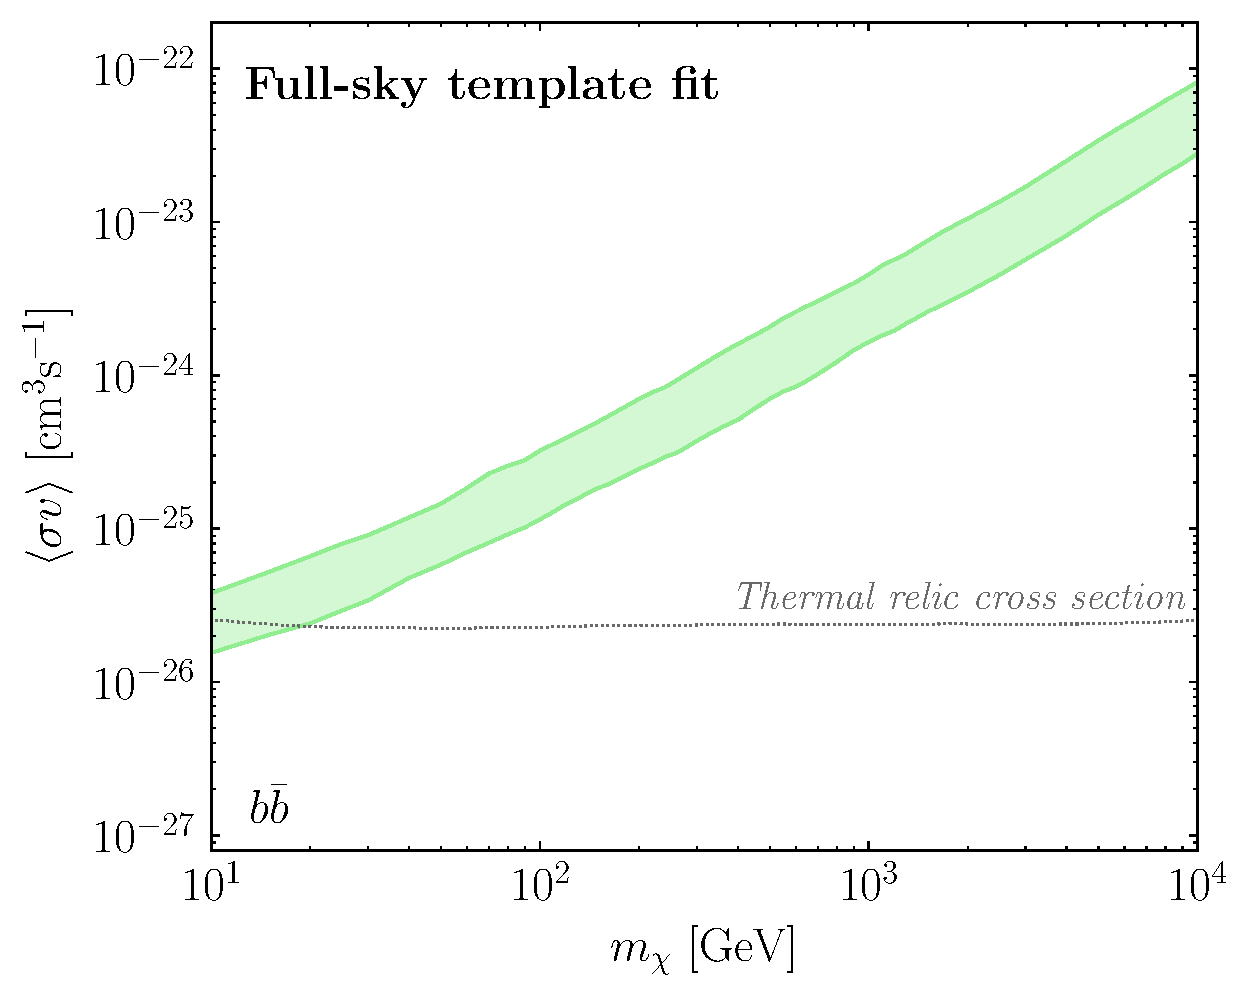
\includegraphics[width=0.45\textwidth]{ch-darksky/plots//TFAllLimitstruth.pdf}
%      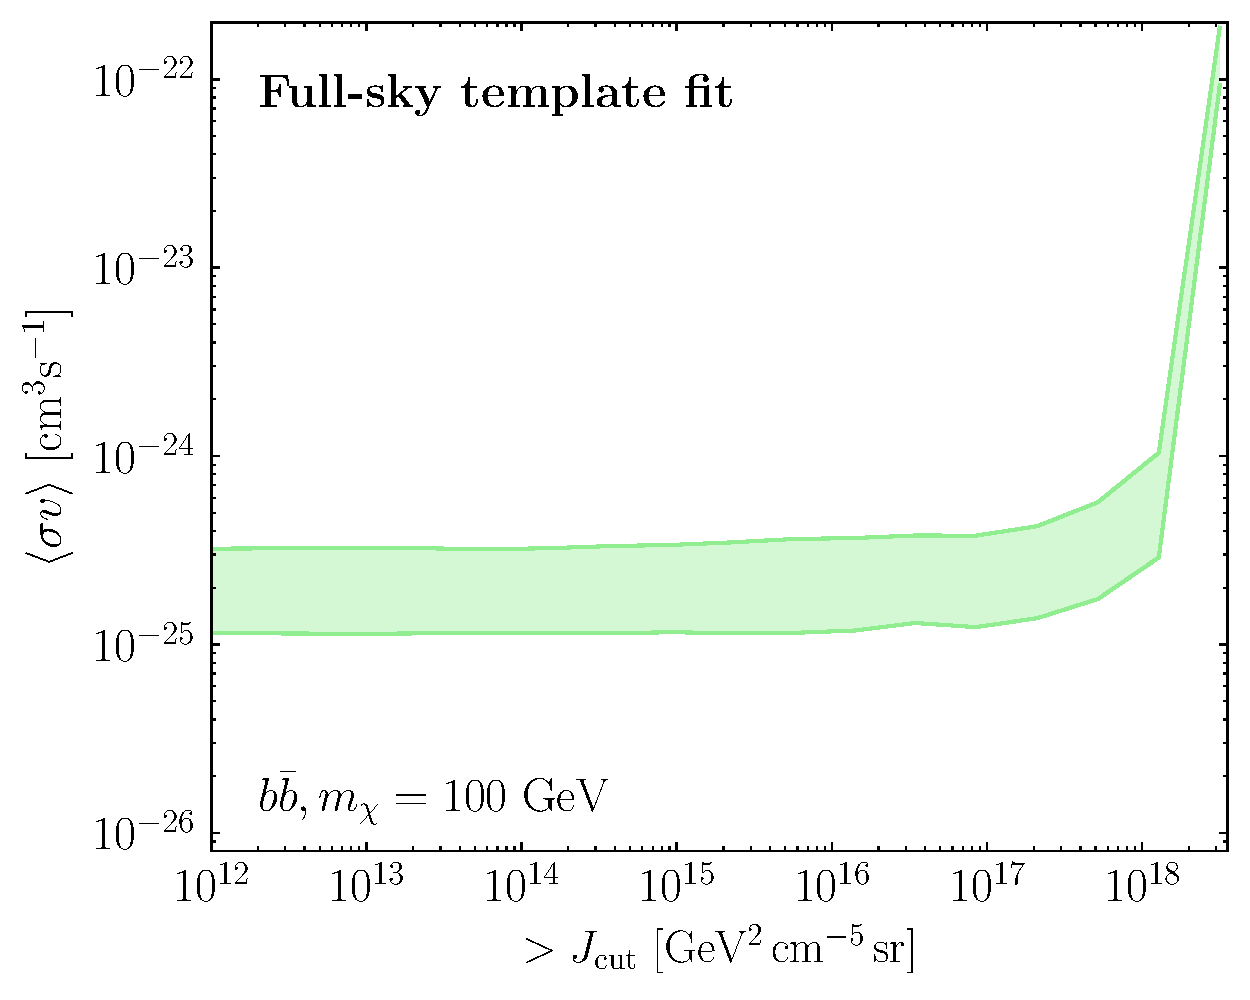
\includegraphics[width=0.45\textwidth]{ch-darksky/plots//TFLimitsJcut.pdf}
%    \caption{ \textbf{(Left)}  The predicted 68\% containment region over 100 MCs for the limit on the annihilation cross section for the full-sky template fitting method.  In this method, all of the $J$-factors from the individual halos are summed together.  Then, the likelihood profile is constructed for the single template.  Note that here we have assumed knowledge of the true $J$-factors, unlike in the previous figures, and have not marginalized over the corresponding uncertainties.
%    \textbf{(Right)}  Projected limits at $m_\chi = 100$~GeV, using the single template-fitting method, as a function of the $J$-factor cut.  Only halos with $J$-factors higher than $> J_\text{cut}$, indicated on the $x$ axis, are included in the analysis.  These results show that the limit is dominated by a small subset of halos with high $J$-factors.
%    }
%    \label{fig:DarkSkyallhalossensitivity}
% \end{figure*}

% One method to alleviate this tension is to impose a maximum energy cut-off.   The right panel of Fig.~\ref{fig:LikelihoodApprox} shows the maximum test statistic, TS$_\text{max}$, of the stacked analysis (for the $b\bar{b}$ channel) for energies below 796~GeV, as a function of DM mass, for data that is a Poisson draw of the background models only.  The green~(yellow) bands show the 68\%~(95\%) spread over 20~MC realizations of the mock data.  We see that TS$_\text{max}$ increases with mass and is inconsistent with 0 at the 95\% level for $m_\chi \gtrsim 500$~GeV.  Note that the 97.5 percentile for TS$_\text{max}$ should be approximately 3.84 assuming a chi-square distribution, though it is over an order of magnitude larger in the MC results at high masses.  To avoid these issues when applying the analysis to real data, we plan to restrict to energies below $\sim$$250$~GeV. The left panel of Fig.~\ref{fig:LikelihoodApprox} shows the TS$_\text{max}$ distribution for energies below 251~GeV, as obtained from 20 MCs of the mock data.  In this case, the simulated TS$_\text{max}$ distribution does a much better, though not perfect, job of approximating the expectation from the chi-square distribution across the $m_\chi$ range.

% A related issue is seen at low DM masses because the approximation we take to the profile likelihood method also breaks down in the lowest energy bins.  In this case, we find that the TS$_\text{max}$ distribution under the null hypothesis does not extend to values as high as would be expected from the chi-square distribution.  In particular, with our default minimum energy of 200 MeV, we find that the 84 and 97.5 percentiles of the TS$_\text{max}$ distribution under the null hypothesis for 10 GeV DM are $\sim$0.14 and $\sim$0.25, respectively.  On the other hand, increasing the minimum energy to 500 MeV brings these values to $\sim$0.70 and $\sim$2.33, respectively, which are in much closer agreement with the expectations from the chi-square distribution.  In Fig.~\ref{fig:LikelihoodApprox}, we implemented the 500 MeV minimum energy and we also plan on using this minimum energy when analyzing the real data.  We suspect that the issues with the lowest energy bins are related to the large PSF at low energies, which can extend the emission from the extragalactic DM halos on the size of the ROI.  This induces degeneracies between the DM template and the astrophysical templates.


% One takeaway from these exercises is that the approximation to the full profile likelihood method discussed here has its limitations.  As a result, it would always be best to perform the full likelihood analysis on the data, if the necessary  computational resources are available.   
% In lieu of that, one can adjust the energy binning to give results that well-approximate the expectations from the exact procedure.
 
 
% \section{Limits Using a Full-Sky Dark Matter Template}
% \label{app:inflimitimpact}

% The main body of this paper presents the results of a stacked analysis in which we analyze individual targets and combine their likelihoods.  Here, we show the results of an analysis where we float the expected emission from all the halos together as a single template.  All resolved point sources are also floated together in this case. The left panel of~Fig.~\ref{fig:DarkSkyallhalossensitivity} shows the projected sensitivity in this case for $b\bar b$ annihilation, \emph{assuming the truth values for the $J$-factors}.  The green band shows the statistical variation of 100 MC iterations of the mock data.  The right panel shows how the limit for $m_\chi = 100$~GeV changes as only halos above a certain $J$-factor threshold are included in the template. Clearly, the sensitivity is dominated by a relatively small number of halos.  This suggests that the normalization of the DM annihilation flux template is being set primarily by the fluctuations of the brightest halos.  We conclude therefore that there is no benefit to doing a full-sky template analysis where the normalizations of all the halos are floated together.  Instead, these results suggest that it is far more advantageous to perform a stacked analysis of the individual galaxy groups, as  explored in this paper. 

\sectionline